%% LyX 1.3 created this file.  For more info, see http://www.lyx.org/.
%% Do not edit unless you really know what you are doing.
\documentclass[english, 12pt]{article}
\usepackage{times}
%\usepackage{algorithm2e}
\usepackage{xurl}
\usepackage{bbm}
\usepackage[T1]{fontenc}
\usepackage[latin1]{inputenc}
\usepackage{geometry}
\geometry{verbose,letterpaper,tmargin=2cm,bmargin=2cm,lmargin=2cm,rmargin=2cm}
\usepackage{rotating}
\usepackage{color}
\usepackage{graphicx}
\usepackage{amsmath, amsthm, amssymb}
\usepackage{setspace}
\usepackage{lineno}
\usepackage{hyperref}
\usepackage{bbm}
\usepackage{makecell}
%\usepackage[font=small]{caption}

\renewcommand{\arraystretch}{1.3}

\usepackage{xr}
\externaldocument{paper-infer-supp}

%\linenumbers
%\doublespacing
\onehalfspacing
\usepackage[authoryear]{natbib}
%\usepackage[numbers,super]{natbib} %\bibpunct{(}{)}{;}{author-year}{}{,}

%Pour les rajouts
\usepackage{color}
\definecolor{trustcolor}{rgb}{0,0,1}

\usepackage{dsfont}
\usepackage[warn]{textcomp}
\usepackage{adjustbox}
\usepackage{multirow}
\usepackage{graphicx}
\graphicspath{{../figures/}}
\DeclareMathOperator*{\argmin}{\arg\!\min}
\usepackage{algorithm}
\usepackage{algpseudocode}

\let\tabbeg\tabular
\let\tabend\endtabular
\renewenvironment{tabular}{\begin{adjustbox}{max width=\textwidth}\tabbeg}{\tabend\end{adjustbox}}

\makeatletter

%%%%%%%%%%%%%%%%%%%%%%%%%%%%%% LyX specific LaTeX commands.
%% Bold symbol macro for standard LaTeX users
%\newcommand{\boldsymbol}[1]{\mbox{\boldmath $#1$}}

%% Because html converters don't know tabularnewline
\providecommand{\tabularnewline}{\\}

\usepackage{babel}
\makeatother


\begin{document}


\title{Inferring disease architecture and predictive ability\\with LDpred2-auto}
\author{Florian Priv\'e,$^{\text{1,}*}$ Clara Albi\~nana,$^{\text{1}}$ Bogdan Pasaniuc,$^{\text{2,3,4,5}}$ and Bjarni J. Vilhj\'almsson$^{\text{1,6,7}}$}

\date{~ }
\maketitle

\noindent$^{\text{\sf 1}}$National Centre for Register-based Research, Aarhus University, Aarhus, Denmark. \\
\noindent$^{\text{\sf 2}}$Bioinformatics Interdepartmental Program, University of California, Los Angeles, CA, USA. \\
\noindent$^{\text{\sf 3}}$Department of Human Genetics, David Geffen School of Medicine, University of California, Los Angeles, CA, USA. \\
\noindent$^{\text{\sf 4}}$Department of Pathology and Laboratory Medicine, David Geffen School of Medicine, University of California, Los Angeles, CA, USA. \\
\noindent$^{\text{\sf 5}}$Department of Computational Medicine, David Geffen School of Medicine, University of California, Los Angeles, CA, USA. \\
\noindent$^{\text{\sf 6}}$Bioinformatics Research Centre, Aarhus University, Aarhus, Denmark. \\
\noindent$^{\text{\sf 7}}$Novo Nordisk Foundation Center for Genomic Mechanisms of Disease, Broad Institute, Cambridge, MA, USA. \\
\noindent$^\ast$To whom correspondence should be addressed. \\

\noindent Contact: \url{florian.prive.21@gmail.com}

%\vspace*{6em}
\clearpage

\begin{abstract}
	
	TODO

\end{abstract}

%%%%%%%%%%%%%%%%%%%%%%%%%%%%%%%%%%%%%%%%%%%%%%%%%%%%%%%%%%%%%%%%%%%%%%%%%%%%%%%%

\clearpage

%%%%%%%%%%%%%%%%%%%%%%%%%%%%%%%%%%%%%%%%%%%%%%%%%%%%%%%%%%%%%%%%%%%%%%%%%%%%%%%%

\section*{Introduction}

Most traits and diseases are heritable. 
What differs is the proportion of phenotypic variance that can be attributable to genetics, i.e.\ the heritability of these phenotypes.
Some phenotypes, such as schizophrenia or height, are highly heritable \cite[]{sullivan2003schizophrenia,yang2010common}. 
These two phenotypes are also highly polygenic, i.e.\ mutations from many genetic variants influences them \cite[]{oconnor2019extreme}.
Understanding how heritable and polygenic a phenotype is can provide valuable clinical insight and inform future research efforts.
Therefore, many methods have been developed to estimate the SNP heritability (referred to as $h^2$ for brevity) and polygenicity ($p$), either globally for the whole genome or locally for specific regions of the genome. 
These methods include GCTA ($h^2$, \cite{yang2011gcta}), BOLT-REML ($h^2$ and $p$, \cite{loh2015contrasting}), LD Score regression ($h^2$, \cite{bulik2015ld}), FINEMAP (per-variant $p$ used for fine-mapping, \cite{benner2016finemap}), HESS (local $h^2$, \cite{shi2016contrasting}), LDAK-SumHer ($h^2$, \cite{speed2019sumher}), S-LD4M ($p$, \cite{oconnor2019extreme}), GRM-MAF-LD ($\alpha$ that can inform about negative selection, \cite{schoech2019quantification}), SuSiE (per-variant $p$ used for fine-mapping, \cite{wang2020simple}), SBayesS ($h^2$, $p$, and a third parameter $S$, similar to $\alpha$, \cite{zeng2021widespread}), and BEAVR (local $p$, \cite{johnson2021estimation}).

As previously shown by \cite{daetwyler2008accuracy}, $h^2$ and $p$ can also be used to determine how well we can predict a phenotype from using genetic variants alone. 
Such genetic predictors are called polygenic scores (PGS), and are getting closer to being included as part of existing clinical risk models for diseases \cite[]{torkamani2018personal,lambert2019towards,kumuthini2022clinical}.
LDpred2 is a widely used polygenic score method that can directly build PGS using summary statistics results from genome-wide associations studies (GWAS), making it highly applicable \cite[]{prive2020ldpred2,pain2021evaluation,kulm2021systematic}.
LDpred2 is a Bayesian approach that uses the SNP heritability $h^2$ and polygenicity $p$ as parameters of its model. In LDpred2-auto, it can directly estimate these parameters from the data, making it applicable even when no validation data is available for tuning these two model hyper-parameters \cite[]{prive2020ldpred2}.

Here we extend LDpred2-auto to make it a highly reliable method for estimating $h^2$ (global and local), $p$ (also per-variant for fine-mapping purposes), and $\alpha$.
So, on top of providing competitive PGS, LDpred2-auto can now provide all these estimates of genetic architecture. 
Moreover, we show how it can now also reliably estimate the predictive ability $r^2$ of PGS it derives, allowing for directly assessing the usefulness of the derived PGS, without needing an independent test set.
An overview of what LDpred2-auto can provide is presented in Figure \ref{fig:overview}.
Finally, we extend the set of HapMap3 variants recommended to use with LDpred2, which enables us to capture around 12\% more SNP heritability and achieve around 6\% more predictive performance $r^2$.
We call this new preferred set of 1,444,196 SNPs HapMap3+.

%%%%%%%%%%%%%%%%%%%%%%%%%%%%%%%%%%%%%%%%%%%%%%%%%%%%%%%%%%%%%%%%%%%%%%%%%%%%%%%%

\begin{figure}[!htb]
	\centerline{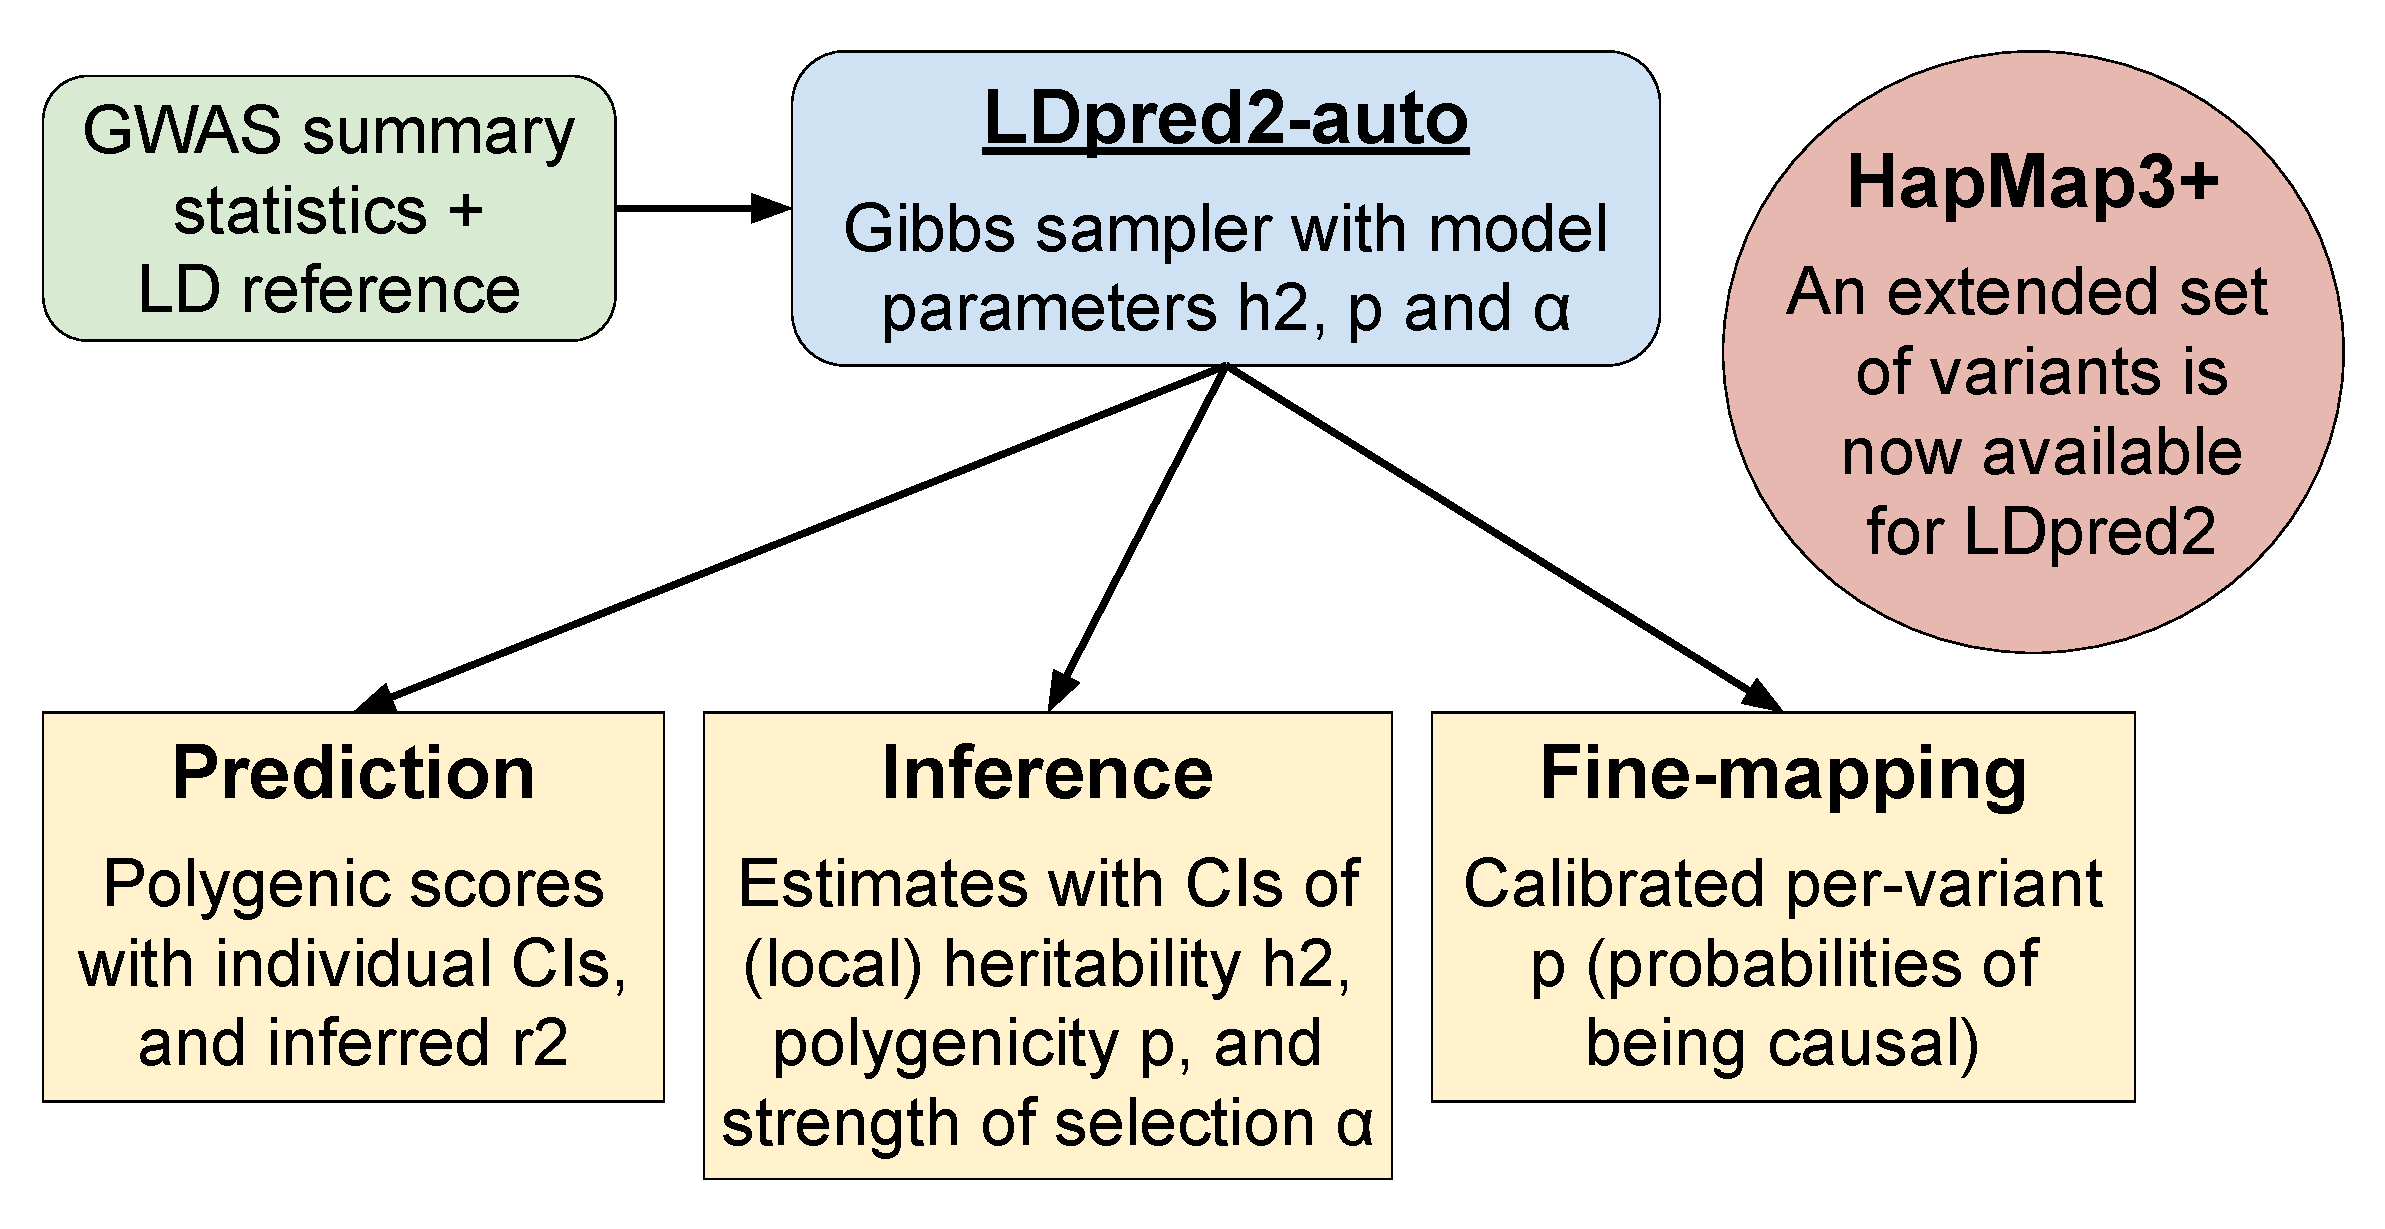
\includegraphics[width=0.8\textwidth]{overview}}
	\caption{Overview of what LDpred2-auto can provide. For individual CIs of polygenic scores, please refer to the work of \cite{ding2022large}. \label{fig:overview}}
\end{figure}



\section*{Results}

[TODO: CHOOSE FIGURES TO HAVE IN MAIN TEXT]

\subsection*{Validating the inference with simulations}

[TODO: INCLUDE SIMPLIFIED VERSIONS OF FIG S1-S3 HERE?]

For simulations, we use the UK Biobank imputed data \cite[]{bycroft2018uk}. We use 356,409 individuals of Northwestern European ancestry and 322,805 SNPs across seven chromosomes (Methods).
We first simulate continuous phenotypes using function \texttt{snp\_simuPheno} from R package bigsnpr \cite[]{prive2017efficient}, varying three parameters: the SNP-heritability $h^2$, the polygenicity $p$ (i.e. the proportion of causal variants), and the parameter $\alpha$ in equation \eqref{eq:new_model} that controls the relationship between minor allele frequencies and expected effect sizes.
This function first picks a proportion $p$ of causal variants at random, sample effect sizes $\gamma$ using the variance component parameterized by $\alpha$ and then scale the effect sizes so that the genetic component $G \gamma$ has a variance $h^2$, where $G$ is the genotype matrix. Finally, some Gaussian noise is added so that the full phenotype has a variance of 1. 
Then, a GWAS is run to obtain summary statistics using $N$ individuals (either the 200,000 dedicated to this, or a subset of 20,000) using a simple linear regression implemented in \texttt{big\_univLinReg} from R package bigstatsr \cite[]{prive2017efficient}.
Finally, we run the new LDpred2-auto model (Methods) with and without the option \texttt{allow\_jump\_sign}, which was proposed in \cite{prive2021identifying} for robustness (when disabled, in which case it prevents effect sizes from changing sign without going through 0 first). 
LDpred2-auto is run with 50 Gibbs sampler chains with different starting values for $p$ (from 0.0001 to 0.2, equally spaced on a log scale).
[TODO: EXPLAIN FILTERING OF CHAINS]

First, LDpred2-auto generally reliably infers the three parameters from its model, i.e.\ the SNP heritability $h^2$, polygenicity $p$, and $\alpha$ (Figures \ref{fig:simu_h2}--\ref{fig:simu_alpha}).
Compared to LD Score regression, heritability estimates are as precise when power is low, and much more precise when power is large, especially for small polygenicity values (Figure \ref{fig:simu_h2}).
When power is low, the polygenicity can be overestimated when the true value is very small (e.g.\ $p=0.0005$), and underestimated when the polygenicity is large (e.g.\ $p=0.1$, Figure \ref{fig:simu_p}).
The $\alpha$ estimate can become unreliable when power is too low, which can be detected by a small number of chains kept from LDpred2-auto (Figure \ref{fig:simu_alpha}).
Then, LDpred2-auto can also infer per-variant probabilities of being causal and per-block (local) heritability estimates, which are well calibrated (Figures \ref{fig:simu_postp_calib} and \ref{fig:simu_h2_calib}).
We recall that calibrated per-variant probabilities of being causal can be used for fine-mapping purposes  \cite[]{wang2020simple}.
Finally, LDpred2-auto can also be used to reliably infer the predictive performance $r^2$ of its resulting polygenic score, directly from within the Gibbs sampler, even when power is low (Figure \ref{fig:simu_r2}).

We then run simulations with binary outcomes where the simulated continuous liabilities are transformed to binary outcomes using a threshold corresponding to the prevalence.
Results are very similar as with the continuous phenotypes above (Figures \ref{fig:simu_h2_bin}--\ref{fig:simu_r2_bin}), and are similar whether we use either a linear regression GWAS and the total sample size $N$, or a logistic regression GWAS and the effective sample size (i.e.\ $N_\text{eff} = 4 / (1 / N_\text{case} + 1 / N_\text{control})$). The only difference is that the $h^2$ and $r^2$ estimates need to be transformed to the liability scale \cite[]{lee2012better}, where $K_\text{GWAS}=0.5$ should be used when using $N_\text{eff}$ in LDpred2-auto or LD Score regression \cite[]{grotzinger2021pervasive}.

 

\subsection*{Genetic architectures of 248 phenotypes from the UK Biobank}

We use the set of 1,054,330 HapMap3 variants recommended to use for LDpred2 \cite[]{prive2020ldpred2}, and the same 356,409 unrelated individuals of Northwestern European ancestry as in the simulations. 
50,000 of these will be used as test set, while the other 306,409 are used to run a GWAS using linear regression (function \texttt{big\_univLinReg}) for each of all 248 phenotypes and using 8 covariates (Methods).
Then the new implementation of LDpred2-auto (Methods) is used.

Consistent with simulations, inferred SNP heritability $h^2$ estimates from LDpred2-auto closely match with those from LD Score regression, while generally being more precise, especially for phenotypes with a smaller polygenicity (Figure \ref{fig:ukbb_h2}).
Note that these $h^2$ estimates (and later the $r^2$ estimates) have not been transformed to the liability scale (i.e.\ are on the observed scale).
Most phenotypes have an estimated polygenicity $p$ between 0.001 and 0.04; these have therefore a very polygenic architecture, but not an infinitesimal one (Figure \ref{fig:ukbb_h2_p}).
Most phenotypes have an estimated $\alpha$ between -1.0 and -0.4 with a mode at -0.65 (Figure \ref{fig:ukbb_h2_alpha}), which is consistent with widespread negative selection.
As for the inferred predictive performance $r^2$, they are highly consistent with the ones derived from the test set; only for standing height and sitting height are they slightly overestimated (Figure \ref{fig:ukbb_r2}). Heritability estimates for these two traits are probably slightly overestimated as well since we use similar formulas for estimating $h^2$ and $r^2$ (Methods), and because the SNP heritability estimate $h^2$ for standing height is higher than values reported in the literature (also see Section ``Application to height''). 

Then, to investigate whether estimates from LDpred2-auto are robust to misspecifications, we test using two alternative LD references (Methods).
Using a smaller number of individuals for computing the LD results in a slightly overestimated $p$ and $h^2$ (and $r^2$), while the $\alpha$ estimate remains consistent, and the predictive performance in the test set remains mostly similar, except for three phenotypes for which none of the LDpred2-auto chains is usable (Figure \ref{fig:small_LD}).
When using an LD reference from an alternative population (South Europe instead of North-West Europe), $p$, $h^2$, and $r^2$ are slightly overestimated as well, and a few phenotypes have lower predictive performance while there are four phenotypes for which none of the LDpred2-auto chains is usable (Figure \ref{fig:alt_LD}).

We then investigate using the extended set of HapMap3 variants proposed here, which includes \textasciitilde40\% more variants than the set of HapMap3 variants recommended to use for LDpred2 (Methods). As expected, compared to HapMap3, higher $h^2$ (average increase of 12.3\% [95\% CI: 10.8, 13.7]) and lower $p$ (decrease of 11.5\% [10.7, 12.3]) estimates are obtained with this extended set HapMap3+ (Figure \ref{fig:hm3_plus}). 
This is consistent with higher predictive performance $r^2$ in the test set (increase of 6.1\% [4.1, 8.2]).
A particularly much larger $h^2$ estimate is obtained for lipoprotein(a) concentration (0.508 [0.502, 0.514] instead of 0.324 [0.320, 0.329]), which is also reflected in a larger predictive performance ($r^2$ in the test set of 0.516 [0.508, 0.524] instead of 0.344 [0.335, 0.353]).
Interestingly, when using this extended set of HapMap3 variants, more chains are kept on average, which is a sign of better convergence of the models (Figure \ref{fig:ukbb_chains}). 
However, fitting with this extended set of variants takes around 50\% more time; yet, we recall that LDpred2 has been made much faster in \cite{prive2021identifying}, and now run in less than one hour for 50 chains parallelized over 13 cores (Figure \ref{fig:ukbb_runtimes}) instead of 4--12 hours before.

Finally, we investigate different transformations to apply to some continuous phenotypes used here.
Indeed, 49 of the phenotypes used here seem log-normally distributed or heavy-tailed (when visualizing their histogram); we therefore log-transform them.
However, we do investigate alternative transformations here to decide which one should be preferred and to check how this impacts the inference from LDpred2-auto.
Note that we now use the HapMap3+ set of variants here.
We first compare to using raw (untransformed) phenotypes in Figure \ref{fig:notransfo}; estimates of $p$ and $\alpha$ are highly consistent.
However, $h^2$ estimates and predictive performance $r^2$ (in the test set) are generally larger with the log-transformation, hinting that it probably makes sense to transform these phenotypes.
We then compare to using the rank-based inverse normal (RIN) transformation in Figure \ref{fig:RINT}; estimates for $p$ and $\alpha$ are also highly consistent.
Except for bilirubin and lipoprotein(a) concentration, generally higher $h^2$ estimates and predictive performance $r^2$ are obtained with the RIN-transformation than the log-transformation.


\subsection*{Local heritability and poligenicity}

In this section, we use the extended set of variants constructed here, HapMap3+, for which we define 431 independent LD blocks (Methods).
We compute per-block (local) $h^2$ estimates, and report the UKBB phenotypes for which one block contributes to at least 10\% of the total heritability of all blocks in Figure \ref{fig:ukbb_local_h2}.
For lipoprotein(a) concentration, ``red hair'' and ``disorders of iron metabolism'' (phecode 275.1), almost all heritability comes from one block only.
We also perform the same analysis with external GWAS summary statistics for 90 cardiovascular proteins \cite[]{folkersen2020genomic}; 22 of them have at least 50\% of their heritability explained by one block, and at least 80\% for 8 of them (Figure \ref{fig:protein_local_h2}). 

Across 169 UKBB phenotypes with more than 25 chains kept, we compute the median heritability per block, and compare it to the number of variants in these blocks; the median heritability explained by a block of variants is largely proportional to the number of variants in this block (Figure \ref{fig:median_local_h2}).
The outlier block explaining a much larger heritability contains the HLA region.
Across the same phenotypes, we then compute per-variant median probabilities of being causal, and report them in a Manhattan-like plot in Figure \ref{median_postp}.
Some variants in multiple small regions across the genome have a larger probability of being causal across many phenotypes; interestingly, these are mapped to genes that are known to be associated with many different traits (up to more than 300) in the GWAS Catalog \cite[]{buniello2019nhgri}.
To verify that this is not driven by population structure, we compute pcadapt chi-square statistics that quantify whether a variant is associated with population structure \cite[]{prive2020performing}; the log-statistics have a negative correlation of -5.5\% with the probabilities of being causal.
To verify that this does not correspond to regions of low LD, we compute LD scores; the probabilities above have a correlation of 11.6\% with the LD scores and of -6.8\% with the log of LD scores.


\subsection*{Application to height}

Here we run three LDpred2-auto models for height, one based on 100K UKBB individuals (as a subset of the 305K used before), one from the same 305K UKBB individuals used before, and one from a large GWAS meta-analysis of 1.6M European individuals [TODO: ADD NUMBER OF VARIANTS] \cite[]{yengo2022saturated}.
Using the method developed in \cite{prive2021using}, we first infer the ancestry proportions of individuals included in the meta-analysis as 81.9\% from N.W. Europe, 9.5\% from E. Europe, 6.5\% from Finland, 1.5\% of Ashkenazi ancestry, 0.3\% from S.W. Europe, and 0.2\% from W. Africa. 
We can therefore use the same N.W. European LD with these GWAS summary statistics. 
Note that we use the HapMap3+ set of 1,444,196 SNPs here, but that we use only 1,013,499 SNPs for the GWAS meta-analysis (those overlapping and passing quality control).

Intercepts from LD Score regression are increasing with sample size: 1.01 (SE: 0.007) with N=100K, 1.11 (0.015) with N=305K, and 2.31 (0.068) with N=1.6M, as expected \cite[]{loh2018mixed}.
SNP heritability estimates are of 65.5\% (SE: 2.8), 59.7\% (2.2), and 39.2\% (1.7) with LD Score regression, respectively. And of 60.2\% [95\% CI: 57.4, 63.1], 62.9\% [61.7, 64.0], and 54.1\% [53.8, 54.4] with LDpred2-auto, respectively.
The reduced heritability estimation from the meta-analysis can be partly explained by three reasons: a reduced number of overlapping SNPs, more heterogeneity in the individuals from the meta-analysis compared to within the UK Biobank only, and less effect of assortative mating (which is strong in the UK Biobank due to the presence of many spouses, and probably contributes to overestimating the heritability of height there).
As expected, predictive performance $r^2$ are increasing with sample size, with 30.0\% [29.2, 30.8], 42.7\% [42.2, 43.1], and 46.9\% [46.8, 47.1], respectively.
Note that the first two estimates (from UKBB) are slightly overestimated, and that the last one is based on a smaller number of overlapping SNPs.
We emphasize that, even though there are 1.6M individuals in the meta-analysis, the predictive performance corresponds to around 87\% of the SNP heritability only (46.9\% versus 54.1\%).
Polygenicity estimates from LDpred2-auto are increasing with sample size with 1.1\% [1.0, 1.4], 2.2\% [2.0, 2.4], and 5.7\% [5.4, 6.0], consistent with results of simulations with a large polygenicity (p=10\%). 
[TODO: RERUN FOR HEIGHT WITH JUMP\_SIGN]
Therefore, we estimate that height has at least 50,000 causal variants.
We also identify 1744 SNPs with a probability of being causal larger than 95\% (fine-mapping).
As for $\alpha$ estimates from LDpred2-auto, they remain highly consistent, with -0.72 [-0.76, -0.68], -0.74 [-0.76, -0.71], and -0.78 [-0.81, -0.75], respectively.
Finally, we compute per-annotation heritability estimates to investigate functional enrichment. We perform this analysis using 50 non-flanking binary annotations from the baselineLD v2.2 model \cite[]{finucane2018heritability}.
Heritability enrichments are rather modest, ranging from 0.7 to 2.5 with a GWAS sample size of N=305K, and of slightly smaller magnitude with N=100K and slightly larger magnitude with N=1.6M (Figure \ref{fig:enrichment}).

%%%%%%%%%%%%%%%%%%%%%%%%%%%%%%%%%%%%%%%%%%%%%%%%%%%%%%%%%%%%%%%%%%%%%%%%%%%%%%%%

\section*{Discussion}

LDpred2-auto was originally developed for building polygenic scores \cite[]{prive2020ldpred2}.
Here we have extended the LDpred2-auto model and shown that it can be used to reliably infer genetic architecture parameters such as the SNP-heritability (global and local), polygenicity (and per-variant probabilities of being causal), and the selection-related parameter $\alpha$.
It can also infer the predictive performance $r^2$ of the resulting PGS (for the same genetic ancestry as the GWAS used for training).
We remind readers that it can also be used to infer the uncertainty of individual polygenic scores \cite[]{ding2022large}.
Results across 248 phenotypes demonstrate that most of these phenotypes are very polygenic, yet do not have an infinitesimal architecture (i.e.\ not all variants are causal); this is consistent with LDpred2-inf generally providing much lower predictive performance than LDpred2-grid or LDpred2-auto \cite[]{prive2020ldpred2}.
We also obtain widespread signatures of selection with most $\alpha$ estimates between -1.0 and -0.4, consistent with previous findings \cite[]{zeng2021widespread}.
However, when looking at the heritability enrichment of several functional annotations for height, we obtain much smaller magnitudes than stratified LD Score regression \cite[]{finucane2018heritability}. For example, \cite{yengo2022saturated} report fold enrichments of more than 10x for e.g.\ coding and conserved variants, while we get less than 2x. 

Here we have also extended the set of HapMap3 variants recommended to use with LDpred2, making it 40\% larger to offer a better coverage of the genome.
This enables us to capture more of the heritability of phenotypes and therefore reduce the missing heritability (i.e.\ the difference between the family-based heritability and the SNP-based heritability).
Using this new set also improves predictive performance here, particularly for lipoprotein(a) concentration with an $r^2$ of 0.516 instead of 0.344.
However, we note that we are able to achieve an $r^2$ of 0.677 [0.671, 0.682] when using the penalized regression implementation of \cite{prive2019efficient} on the UKBB individual-level data while restricting to all variants within a 1Mb window of the \textit{LPA} gene.
It means that this extended SNP set is still not tagging all variants perfectly, and that it might be preferable to use a more targeted set of variants for phenotypes for which most of the heritability is contained in a single region of the genome.

Our proposed method has limitations. First, when power is low, estimates of $\alpha$ and $p$ become less reliable. However, estimates of $h^2$ and $r^2$ seem always reliable, except for maybe height for which they are probably overestimated.
We think this is likely due to assortative mating \cite[]{border2022assortative,yengo2022saturated}. 
Moreover, the $h^2$ from LDpred2-auto is also slightly overestimated when using a small LD reference panel or when the reference panel does not closely match with the ancestry of the GWAS summary statistics; future work could focus on correcting this issue. [TODO: OTHERS?]

Nevertheless, LDpred2-auto users can now get much from running a single method only. The reliable estimates provided by LDpred2-auto are very encouraging to further extend LDpred2-auto in multiple directions. 
As future research directions, we are interested in using LDpred2-auto for GWAS summary statistics imputation \cite[]{rueger2018evaluation,julienne2019raiss}, for genetic correlation estimation \cite[]{bulik2015atlas,shi2017local,speed2019sumher,frei2019bivariate,werme2022integrated}, multi-ancestry prediction and inference \cite[]{brown2016transethnic,shi2020localizing,ruan2022improving,lu2022multi}, as well as extending it to learn from functional annotations \cite[]{zhang2021improved,marquez2021incorporating}.

%%%%%%%%%%%%%%%%%%%%%%%%%%%%%%%%%%%%%%%%%%%%%%%%%%%%%%%%%%%%%%%%%%%%%%%%%%%%%%%%

\section*{Materials and Methods}

\subsection*{Data for simulations}

For simulations, we use the UK Biobank imputed (BGEN) data, read as allele dosages with function \texttt{snp\_readBGEN} from R package bigsnpr \cite[]{bycroft2018uk,prive2017efficient}. 
We use the set of 1,054,330 HapMap3 variants recommended to use for LDpred2 \cite[]{prive2020ldpred2}.
Since we run lots of different models, we restrict the simulations to chromosomes 3, 6, 9, 12, 15, 18 and 21, resulting in a set of 322,805 SNPs.
We restrict individuals to the ones used for computing the principal components (PCs) in the UK Biobank (field 22020). These individuals are unrelated and have passed some quality control including removing samples with a missing rate on autosomes larger than 0.02, having a mismatch between inferred sex and self-reported sex, and outliers based on heterozygosity (more details can be found in section S3 of \citet{bycroft2018uk}).
To get a set of genetically homogeneous individuals, we compute a robust Mahalanobis distance based on the first 16 PCs (field 22009) and further restrict individuals to those within a log-distance of 4.5 \cite[]{prive2020efficient}.  
This results in 356,409 individuals of Northwestern European ancestry.
We randomly sample 200,000 individuals to form a training set (to run the GWAS), and use the remaining individuals to form a test set (to evaluate the predictive models).

\subsection*{Data for the UK Biobank analyses}

We use the set of 1,054,330 HapMap3 variants recommended to use for LDpred2 \cite[]{prive2020ldpred2}, and the same 356,409 individuals of Northwestern European ancestry as in the simulations.
We randomly sample 50,000 individuals to form a test set (to evaluate the predictive models), and use the remaining individuals to form a training set (to run the GWAS).

We construct and use the same phenotypes as in \cite{prive2021high}. [TODO: PROVIDE THE LIST SOMEWHERE]
About half of these consists of phecodes mapped from ICD10 and ICD9 codes using R package PheWAS \cite[]{carroll2014r,wu2019mapping}.
The other half consists of phenotypes defined in UKBB fields based on manual curation \cite[]{prive2021high}.
As covariates, for the subset of individuals previously defined, we first recompute PCs using function \texttt{snp\_autoSVD} from R package bigsnpr and keep four PCs based on visual inspection \cite[]{prive2017efficient,prive2020efficient}. We also use sex (field 22001), age (field 21022), birth date (combining fields 34 and 52) and deprivation index (field 189) as additional covariates.


We use the LD matrix with independent LD blocks computed in \cite{prive2021identifying}.
We design two other LD matrices: one using a smaller subset of 2000 individuals from the previously selected ones (which we call ``hm3\_small''), and one based on 10,000 individuals from around South Europe by using the ``Italy'' center defined in \cite{prive2021high} (``hm3\_altpop'').
We apply the optimal algorithm developed in \cite{prive2021optimal} to obtain independent LD blocks, as recommended in \cite{prive2021identifying}.
We finally define a fourth LD reference by extending the set of HapMap3 variants (see next Methods section) and using 20,000 individuals from the previously selected ones (``hm3\_plus'').

\subsection*{Extending the set of HapMap3 variants used}

The HapMap3 variants generally provide a good coverage of the whole genome.
We recall that the set of 1,054,330 HapMap3 variants recommended to use for LDpred2 \cite[]{prive2020ldpred2} is a subset of the original set of HapMap3 variants, which does not include duplicated positions (e.g.\ multi-allelic variants), nor ambiguous variants (e.g.\ both 'A' and 'T' or 'C' and 'G'), and which includes SNPs only (e.g.\ no indel).
Here we propose to extend the set we have used for LDpred2 until then. 
This extension aims at making sure many genetic variants are well tagged by the extended set.
To design this new set, we first read all variants from the UK Biobank (UKBB) with a minor allele frequency (MAF) larger than 0.005 in the whole data (i.e.\ the MAF from the MFI files). 
We then compute all pairwise correlations between variants within a 1 Mb distance, restricting to squared correlations larger than 0.3, and using all unrelated UKBB individuals excluding all White British (field 22006) to have a set of individuals from diverse ancestries.
Finally, we design an algorithm which aims at maximizing the tagging of all these variants read. We want to maximize $\sum_j \max_{k \in \text{HapMap3+}} r_{j,k}^2$, where $j$ spans the whole set of variants read, while $k$ spans the variants kept in the new set, which we call HapMap3+.
We start by including all previously used HapMap3 variants.
Then, for the sake of simplicity, we use a greedy approach, where we repeatedly include the variant which increases this sum most, until no variant improves it by more than 2. 
Note that we only allow non-ambiguous SNPs to be included.
This results in an extended set of 1,444,196 SNPs, of which we compute the correlation between variants (within a 3 cM window) and apply the optimal algorithm developed in \cite{prive2021optimal} to obtain 431 independent LD blocks.

\subsection*{New model and inference with LDpred2-auto}

LDpred2 originally assumed the following model for effect sizes,
\begin{equation}\label{eq:prev_model}
\beta_j = S_j \gamma_j \sim \left\{
\begin{array}{ll}
\mathcal N\left(0,~\dfrac{h^2}{M p}\right) & \mbox{with probability $p$,} \\
0 & \mbox{otherwise,}
\end{array}
\right.
\end{equation}
where $p$ is the proportion of causal variants, $M$ the number of variants, $h^2$ the (SNP) heritability, $\gamma$ the effect sizes on the allele scale, $S$ the standard deviations of the genotypes, and $\beta$ the effects of the scaled genotypes \cite[]{prive2020ldpred2}.
In LDpred2-auto, $p$ and $h^2$ are directly estimated within the Gibbs sampler, as opposed to testing several values of $p$ and $h^2$ from a grid of hyper-parameters. This makes LDpred2-auto a method free of hyper-parameters which can therefore be applied directly to data without the need of a validation dataset to choose best-performing hyper-parameters \cite[]{prive2020ldpred2}.
Previously, $p$ was sampled from $\text{Beta}(1 + M_c, 1 + M - M_c)$, where $M_c = \sum_j(\beta_j \neq 0)$.

Here we introduce a few changes to LDpred2-auto, which makes it better at inferring these important parameters.
First, we extend LDpred2-auto with a third parameter $\alpha$ that controls the relationship between minor allele frequencies (or equivalently, standard deviations) of genotypes and expected effect sizes; the model becomes
\begin{equation}\label{eq:new_model}
\beta_j = S_j \gamma_j \sim \left\{
\begin{array}{ll}
\mathcal N \big( 0,~\sigma_\beta^2 \cdot (S_j^2)^{(\alpha + 1)} \big) & \mbox{with probability $p$,} \\
0 & \mbox{otherwise.}
\end{array}
\right.
\end{equation}
Therefore, it was earlier assumed that $\alpha = -1$ and $\sigma_\beta^2 = h^2 / (M p)$ in equation \eqref{eq:prev_model}. 
This new model in equation \eqref{eq:new_model} is similar to the model assumed by SBayesS, where $\alpha$ is called $S$ \cite[]{zeng2021widespread}. 
In SBayesS, they estimate $\alpha$ and $\sigma_\beta^2$ by maximizing the likelihood of the normal distribution (over the causal variants from the Gibbs sampler).
In the new LDpred2-auto, we first sample causal variants with replacement (bootstrap) before computing the maximum likelihood estimators, such that we add some proper sampling to these two parameters. 
This maximum likelihood estimation is implemented using R package roptim \cite[]{pan2020roptim}, and we bound the estimate of $\alpha$ to be between -1.5 and 0.5 (the default, but can be modified), and the estimate of $\sigma_\beta^2$ to be between 0.5 and 2 times the one from the previous iteration.
We now sample $p$ from $\text{Beta}(1 + M_c / \bar{l^2}, 1 + (M - M_c) / \bar{l^2})$, where $\bar{l^2}$ is the average LD score, to add more sampling by properly accounting for the reduced effective number of correlated variants.
As for $h^2$, we still estimate it by $h^2 = \boldsymbol{\beta}^T \boldsymbol{R} \boldsymbol{\beta}$, where $\boldsymbol{R}$ is the correlation matrix between variants and $\boldsymbol{\beta}$ is a vector of causal effect sizes (after scaling) from one iteration of the Gibbs sampler. 
We constrain this estimate to be at least 0.001 to prevent the Gibbs sampler from being trapped in very small heritability estimates.
Note that this $h^2$ estimate can be restricted to e.g.\ variants from a single LD block to get estimates of local heritability.

\subsection*{Inference of predictive performance from the Gibbs sampler}

[TODO: EXPLAIN HOW TO INFER R2]

[MENTION PARTIAL COR?]

%%%%%%%%%%%%%%%%%%%%%%%%%%%%%%%%%%%%%%%%%%%%%%%%%%%%%%%%%%%%%%%%%%%%%%%%%%%%%%%%


\clearpage
%\vspace*{3em}

\section*{Acknowledgements}

Authors thank members of the NCRR/QGG StatGen group for helpful discussions.
Authors also thank GenomeDK and Aarhus University for providing computational resources and support that contributed to these research results.
This research has been conducted using the UK Biobank Resource under Application Number 58024; authors thank all the UK Biobank participants for contributing to such useful data for Research.

\section*{Funding}

F.P., C.A.\ and B.J.V.\ are supported by the Danish National Research Foundation (Niels Bohr Professorship to Prof.\ John McGrath), the Lundbeck Foundation Initiative for Integrative Psychiatric Research, iPSYCH (R102-A9118, R155-2014-1724, R248-2017-2003), and a Lundbeck Foundation Fellowship (R335-2019-2339 to B.J.V.).

\section*{Declaration of Interests}

B.J.V.\ is on Allelica's international advisory board.
The other authors have no competing interests to declare.

\section*{Code and data availability}

The UK Biobank data is available through a procedure described at \url{https://www.ukbiobank.ac.uk/using-the-resource/}. 
All code used for this paper is available at \url{https://github.com/privefl/paper-infer/tree/master/code}.
We have extensively used R packages bigstatsr and bigsnpr \cite[]{prive2017efficient} for analyzing large genetic data, packages from the future framework \cite[]{bengtsson2020unifying} for easy scheduling and parallelization of analyses on the HPC cluster, and packages from the tidyverse suite \cite[]{wickham2019welcome} for shaping and visualizing results.
The latest version of R package bigsnpr can be installed from GitHub.%, and a recent enough version can be installed from CRAN [TODO: VERIFY].

\noindent[TODO: TABLE EXPORTING RESULTS (ESTIMATES)]

\noindent[TODO: EXPORT LDREF FOR NEW HAPMAP3+]

\noindent[TODO: UPDATE LDPRED2 TUTORIAL TO INCLUDE INFERENCE]

%%%%%%%%%%%%%%%%%%%%%%%%%%%%%%%%%%%%%%%%%%%%%%%%%%%%%%%%%%%%%%%%%%%%%%%%%%%%%%%%

\clearpage
%\vspace*{3em}

\bibliographystyle{natbib}
\bibliography{refs}

%%%%%%%%%%%%%%%%%%%%%%%%%%%%%%%%%%%%%%%%%%%%%%%%%%%%%%%%%%%%%%%%%%%%%%%%%%%%%%%%


\end{document}
